\message{ !name(paper.tex)}%  article.tex (Version 3.3, released 19 January 2008)
%  Article to demonstrate format for SPIE Proceedings
%  Special instructions are included in this file after the
%  symbol %>>>>
%  Numerous commands are commented out, but included to show how
%  to effect various options, e.g., to print page numbers, etc.
%  This LaTeX source file is composed for LaTeX2e.

%  The following commands have been added in the SPIE class 
%  file (spie.cls) and will not be understood in other classes:
%  \supit{}, \authorinfo{}, \skiplinehalf, \keywords{}
%  The bibliography style file is called spiebib.bst, 
%  which replaces the standard style unstr.bst.  

\documentclass[]{spie}  %>>> use for US letter paper
%%\documentclass[a4paper]{spie}  %>>> use this instead for A4 paper
%%\documentclass[nocompress]{spie}  %>>> to avoid compression of citations
%% \addtolength{\voffset}{9mm}   %>>> moves text field down
%% \renewcommand{\baselinestretch}{1.65}   %>>> 1.65 for double spacing, 1.25 for 1.5 spacing 
%  The following command loads a graphics package to include images 
%  in the document. It may be necessary to specify a DVI driver option,
%  e.g., [dvips], but that may be inappropriate for some LaTeX 
%  installations. 
\usepackage[]{graphicx}

\title{Texture mapping 3D planar models of indoor environments with noisy camera poses} 

%>>>> The author is responsible for formatting the 
%  author list and their institutions.  Use  \skiplinehalf 
%  to separate author list from addresses and between each address.
%  The correspondence between each author and his/her address
%  can be indicated with a superscript in italics, 
%  which is easily obtained with \supit{}.

\author{Peter Cheng, Michael Anderson, Stewart He, Avideh Zakhor
\skiplinehalf
University of California, Berkeley\\
}

 

%%%%%%%%%%%%%%%%%%%%%%%%%%%%%%%%%%%%%%%%%%%%%%%%%%%%%%%%%%%%% 
%>>>> uncomment following for page numbers
% \pagestyle{plain}    
%>>>> uncomment following to start page numbering at 301 
%\setcounter{page}{301} 
 
\begin{document}

\message{ !name(paper.tex) !offset(106) }
\subsection{Direct Mapping}
\label{sec:directMapping}

Ignoring the fact that the camera matrices $P_{1..M}$ are inaccurate,
we can texture the plane by discretizing it into small square tiles,
in our case 5 pixels across, and choosing an image to texture each
tile.

We choose to work with rectangular units to ensure that borders
between any two distinct images in the final texture are either
horizontal or vertical. Since most strong environmental features
inside buildings are horizontal or vertical, any visible seams in our
texture intersect them minimally and are less noticeable.

In order to select an image for texturing a tile $t$, we must first
gather a list of candidate images that contain all four of its
corners, which we can quickly check by projecting $t$ into each image
using the $P_i$ camera matrices. Furthermore, each candidate image
must have been taken at a time when its camera had a clear
line-of-sight to $t$, which can be calculated using standard
ray-polygon intersection tests between the camera location, $t$, and
every other plane \cite{rayintersection}.

Once we have a list of candidate images for $t$, we define a scoring
function in order to objectively select the best image for texturing
$t$. Since camera pose errors compound over distance, we wish to
minimize the distance between cameras and the surfaces they
texture. Additionally, we desire images that are projected
perpendicularly onto the plane, maximizing the resolution and amount
of useful texture available in their projections, as well as
minimizing any parallax effects due to real-world geometry not
represented by our digital model. In other words, we wish to minimize
the angle between the tile's normal vector and the camera axis for
images selected for texture mapping. These two criteria can be met by
maximizing the function $\frac{1}{d} (-1 \cdot \vec{c}) \cdot \vec{n}$
as shown in Figure \ref{fig:scoringFunction}. Specifically, $d$ is the
distance between the centers of a camera and a tile, and $\vec{n}$ and
$\vec{c}$ are the directions of the plane's normal and the camera axis
respectively.

\begin{figure}
  \centering
  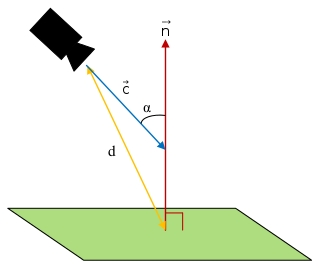
\includegraphics[height=1.5in]{scoringFunction.jpg}
  \caption{We minimize camera angle $\alpha$ and distance $d$ by
    maximizing the scoring function $\frac{1}{d} (-1 \cdot \vec{c})
    \cdot \vec{n}$}
  \label{fig:scoringFunction}
\end{figure}



\begin{figure}[h!]
  \centering \subfloat[][]{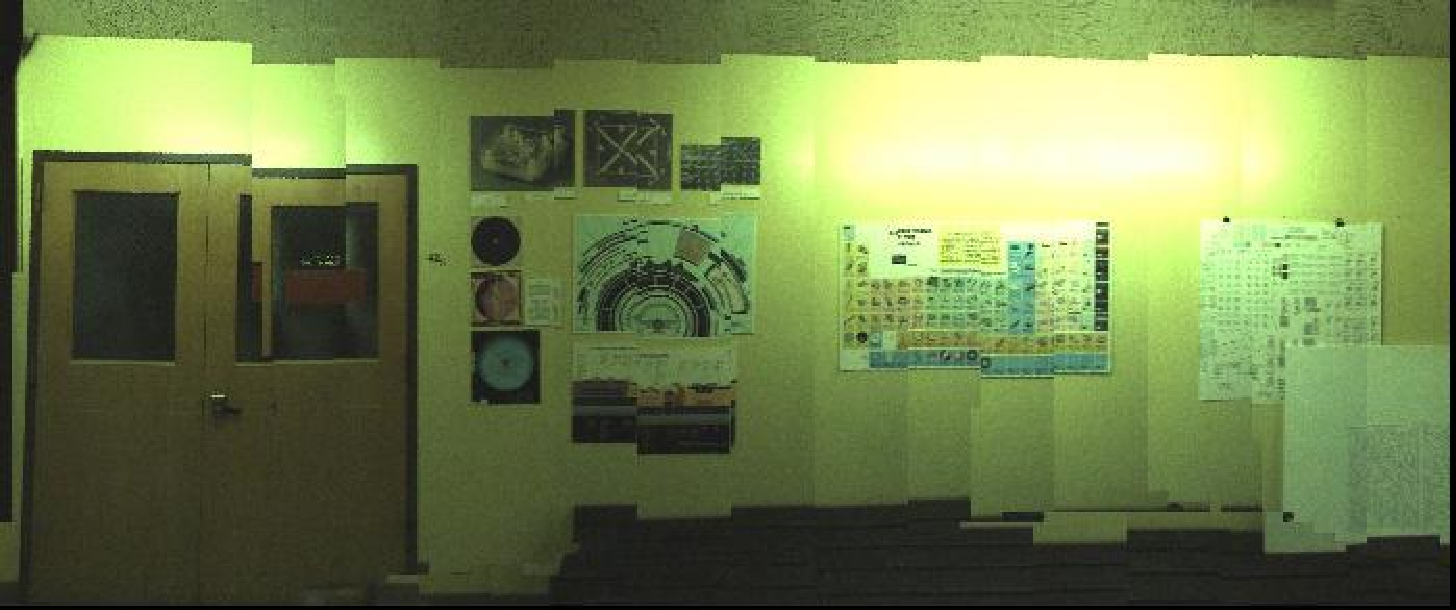
\includegraphics[width=3in,
    height=0.97in]{wall2_naive.pdf}}

  \centering \subfloat[][]{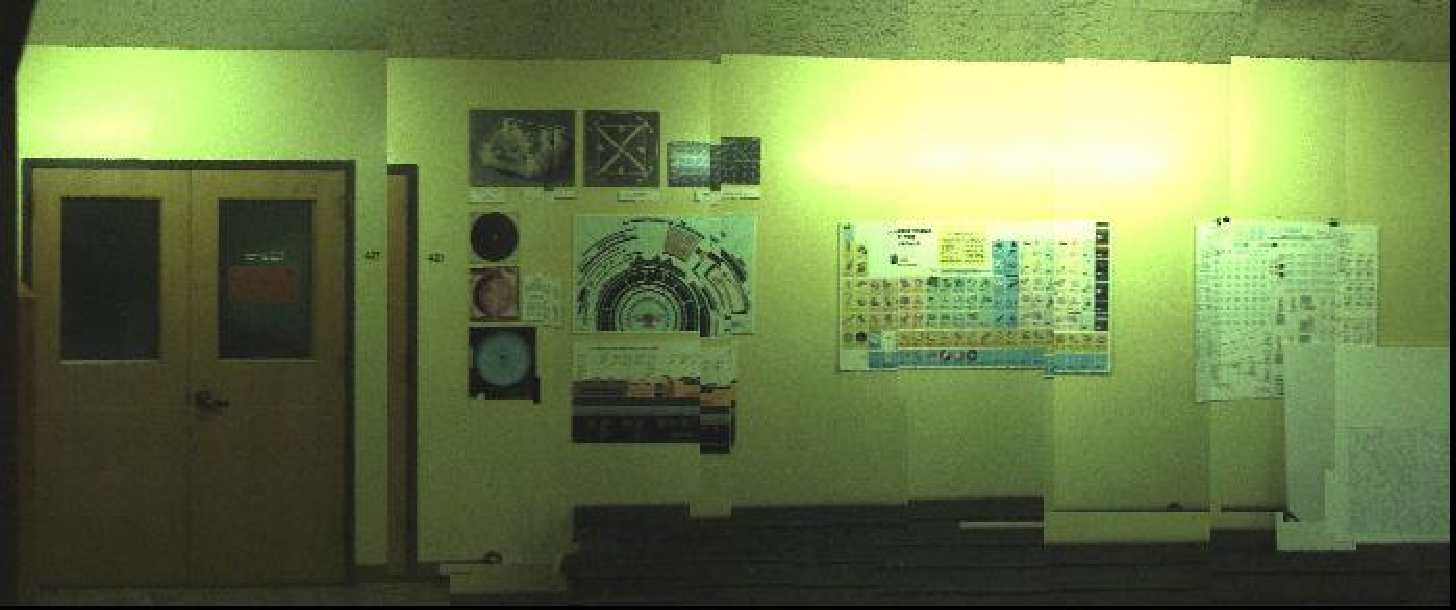
\includegraphics[width=3in,
    height=0.97in]{wall2_cache.pdf}}

  \centering \subfloat[][]{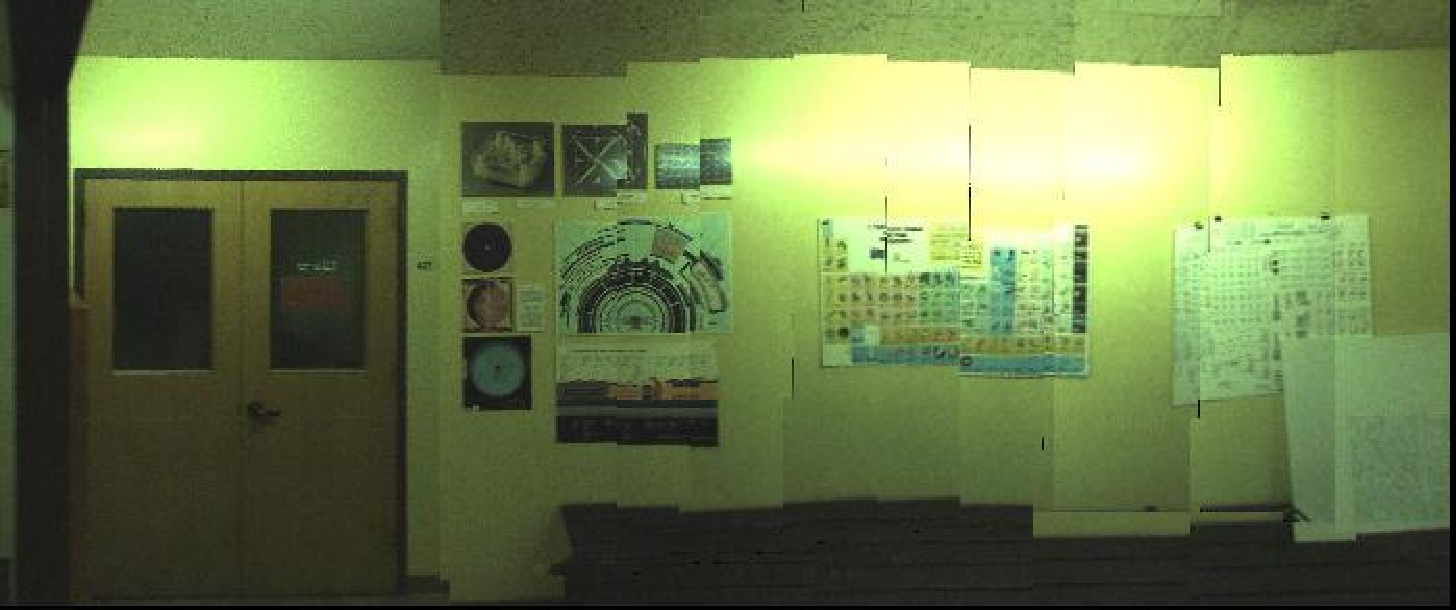
\includegraphics[width=3in,
    height=0.97in]{wall2_cache_shift.pdf}}

  \centering \subfloat[][]{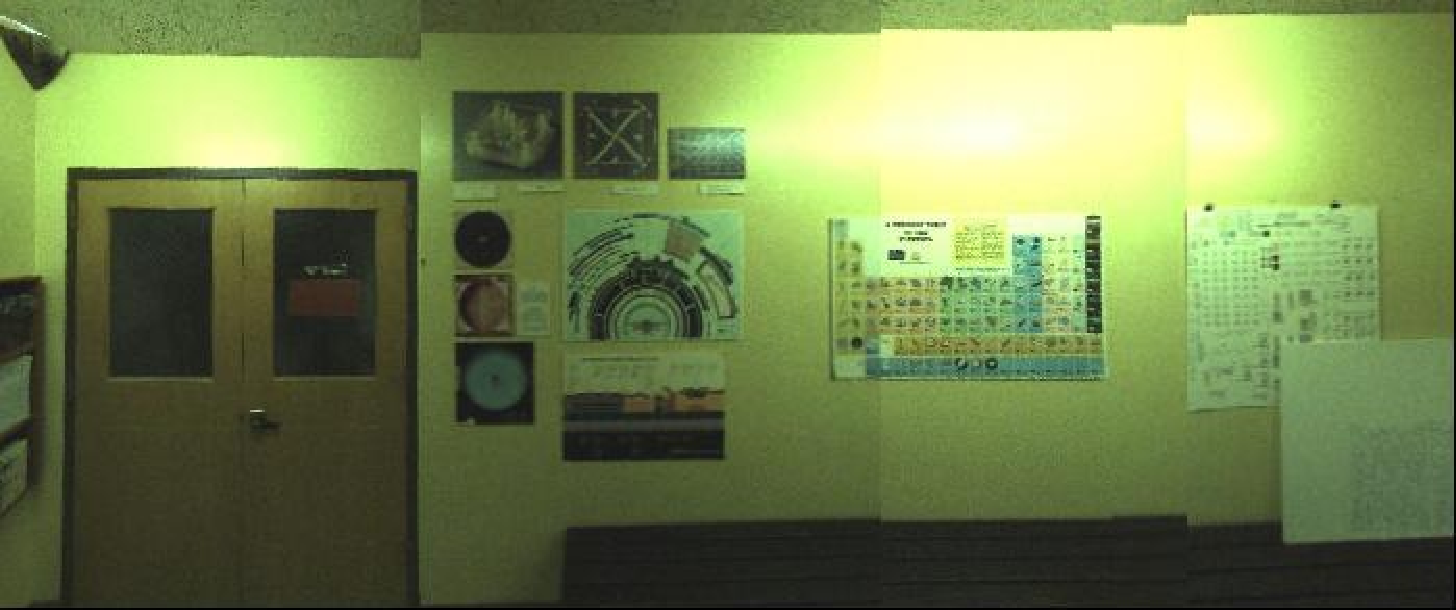
\includegraphics[width=3in,
    height=0.97in]{wall2_dynprog_noblend.pdf}}

  \centering \subfloat[][]{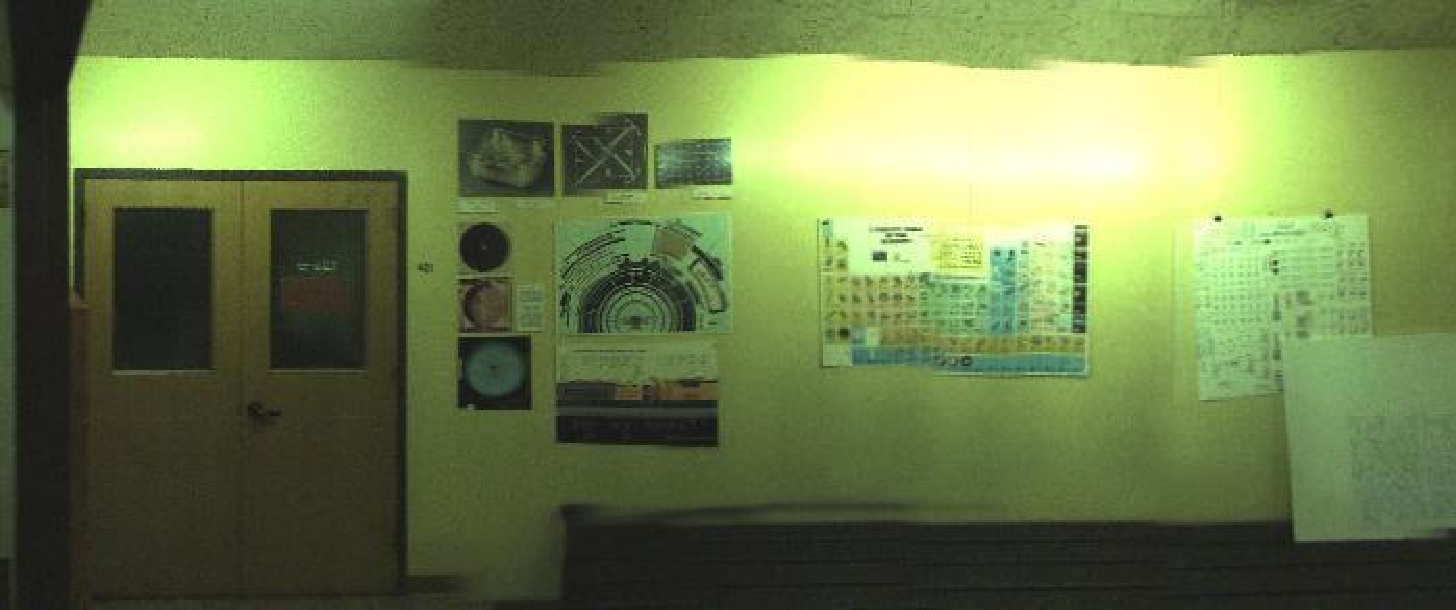
\includegraphics[width=3in,
    height=0.97in]{wall2_cache_shift_blend.pdf}}

  \centering \subfloat[][]{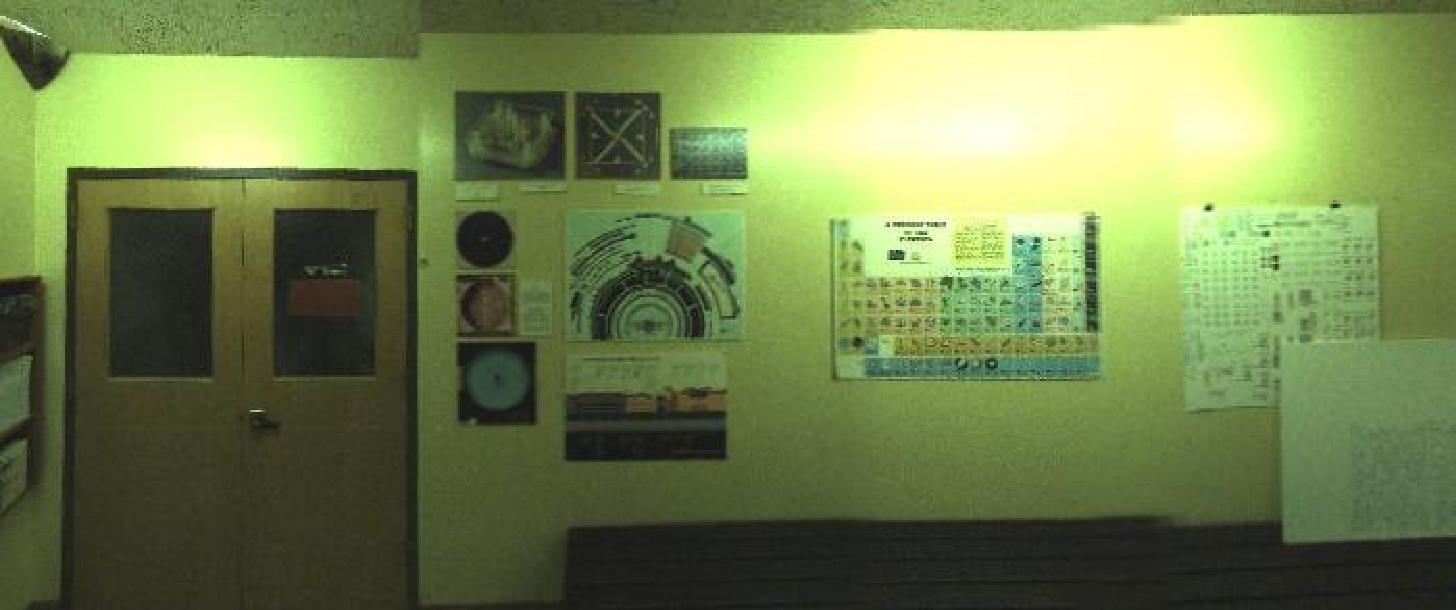
\includegraphics[width=3in,
    height=0.97in]{wall2_dynprog.pdf}}
  \caption{(a) Direct mapping. (b) Mapping with caching. (c) Mapping
    with caching after image alignment. (d) Seam minimization after
    image alignment). (e) same as (c) with blending. (f) same as (d)
    with blending.}
  \label{fig:compareAll}
\end{figure}


As Figure \ref{fig:compareAll}(a) demonstrates, this approach leads to
the best texture for each tile independently, but overall results in
many image boundaries with abrupt discontinuities, due to significant
misalignment between images, as a result of camera pose inaccuracies.



\message{ !name(paper.tex) !offset(416) }

\end{document} 
